\section{ESTRUCTURACION}

Debido a la distribución dispuesta en los planos de arquitectura, se ha optado por una estructuración tipo muro. A continuación, se adjuntan dos imágenes que muestran la distribución de espacios y la ubicación de los elementos estructurales.

\begin{figure}[h]
    \centering
    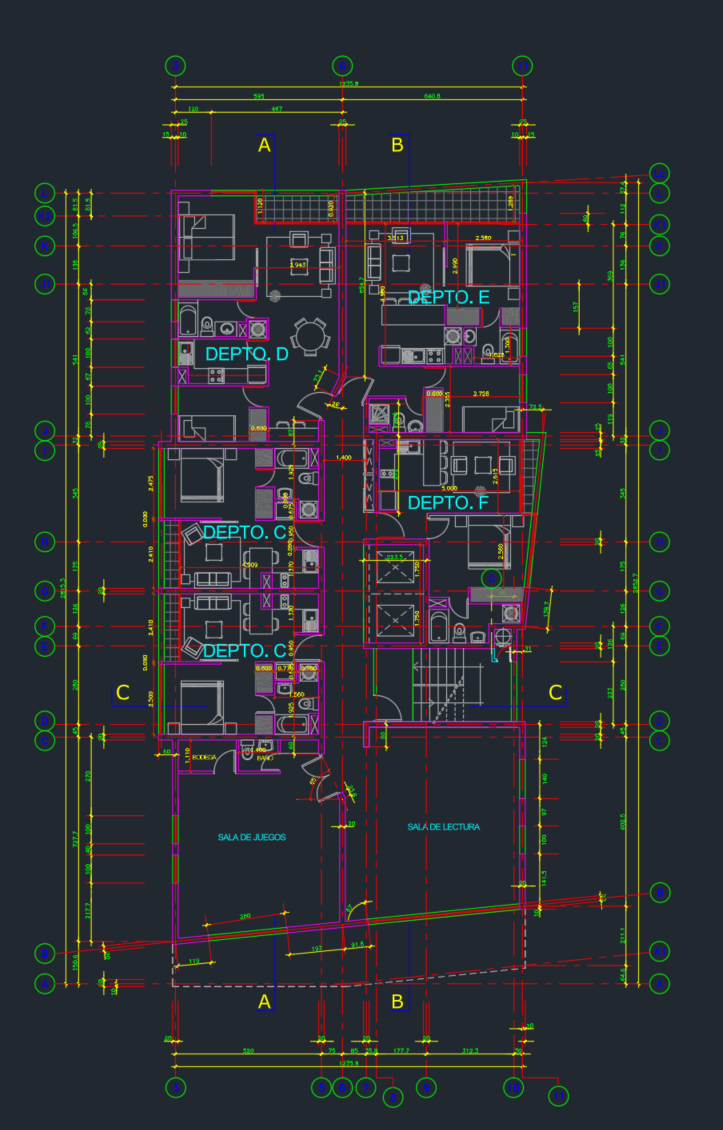
\includegraphics[width=0.45\textwidth]{secciones_inf/IMG/Plano_1.png}
    \caption{Distribución de espacios y elementos estructurales}
\end{figure}

Además, la estructura se compondrá de dos nucleos que serán la caja escala y donde están ubicados los ascensores. Estos nucleos brindarán estabilidad, rigidez y resistencia a la estructura frente a cargas laterales, como las provocadas por el viento o los sismos.

También, las columnas que se ubicarán principalmente en los estacionamientos, ya que en el resto del edificio se ha optado por una estructuración tipo muro. Estas columnas ayudarán a soportar las cargas verticales de el primer piso dando espacio para que los autos circulen en el estacionamiento del subsuelo.

Otro elemento estructural que se ha considerado son las vigas, eso sí, en ubicaciones específicas para proporcionar soporte adicional a las losas y distribuir las cargas de manera eficiente. 

Además, se ocuparán losas de concreto armado para las diferentes plantas del edificio, lo que contribuirá a soportar las cargas verticales del edificio.

Finalmente, en cuanto a fundaciones se van a ocupar diferentes tipos, ya que en el subsuelo van a haber muros y columnas. Por lo tanto, se van a ocupar zapatas aisladas para las columnas y zapatas corridas para los muros.   

